\section{Parameter analysis}
% Introduce the analysis of the different parameters, and show that in this chapter we will see how changing each parameter can influence different parts of the system.

% Terrain generation
% Show how the different parameters of noise generation influence the resulting heightmap

% Curve planner
% Background already discusses the parameters. Compare this with own experiments

% Pdd generator
% show the impact of radius and density.
\subsection{Pdd placement and object density}
In the PDD placement algorithm the placement of the objects is dependent on the radius of each layer. Changing the radius of an object changes the minimum distance between two objects. The density of the objects placed can therefore be changed by increasing the radius. To show the effect of the radius on the density, we take an initial radius $r$ that represents the bounds of the object itself. We increase this radius by a factor $f$ and run the algorithm. From the amount of points placed we calculate the area that the points occupy with the original radius, and calculate the density. To see the effect of increasing the radius of an object, we take a range from 1 to 4, with increments of 0.2. For each ratio, we run the algorithm 500 times, and calculate the density by calculating the circular area of the initial radius. The results of this example are shown in figure \ref{fig:pdd-parameters-example}, along with a few examples showing the change of radius. The blue bars show the results of the experiment, and the orange line is an exponential distribution, fitted on the data. From this we can see that the density generally follows an exponential distribution. In the examples we can see that increasing the layer radius reduces the places that objects can be placed. % Should probably write more.


\begin{figure}
    \begin{subfigure}{.5\textwidth}
        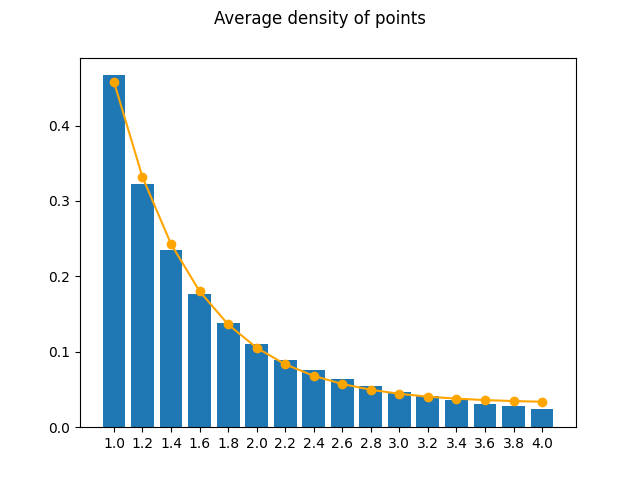
\includegraphics[width=\linewidth]{figures/parameters/pdd-parameters-graph.png}
    \end{subfigure}
    \begin{subfigure}{.5\textwidth}
        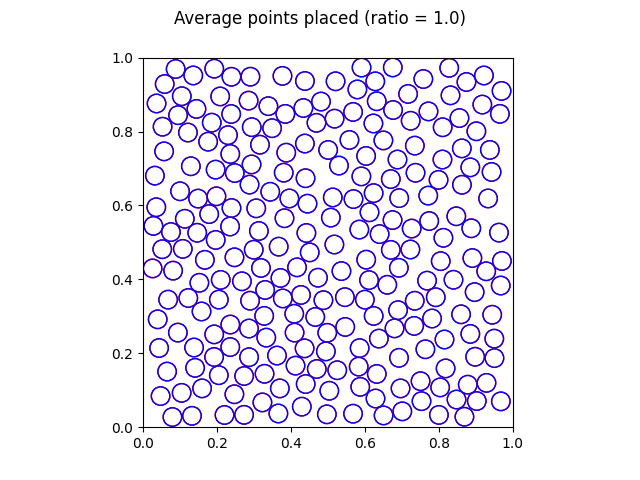
\includegraphics[width=\linewidth]{figures/parameters/pdd-parameters-example-1.png}
    \end{subfigure}
    \begin{subfigure}{.5\textwidth}
        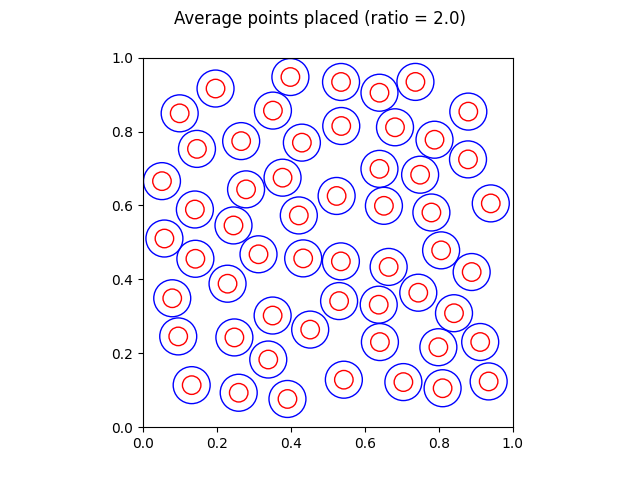
\includegraphics[width=\linewidth]{figures/parameters/pdd-parameters-example-2.png}
    \end{subfigure}
    \begin{subfigure}{.5\textwidth}
        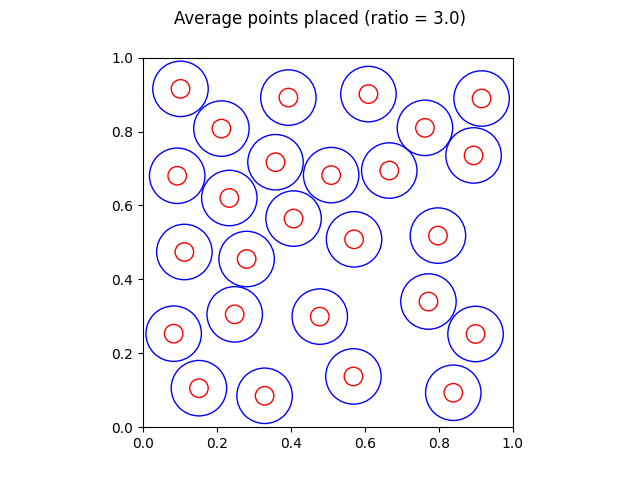
\includegraphics[width=\linewidth]{figures/parameters/pdd-parameters-example-3.png}
    \end{subfigure}
    \caption{Graph of the influence of radius on density, and examples of increasing the radius (blue) on an initial radius (red)}
    \label{fig:pdd-parameters-example}
\end{figure}

